%----------------------------------------------------------------------------
\chapter{Design}
%----------------------------------------------------------------------------
\section{Goals}
My goal is to implement a tool in LabVIEW, which can provide test inputs for a single VI, its front panel controls or input terminals. These test inputs should cover all the possible execution paths (in the case of LabVIEW, all the subdiagrams, or all combination of subdiagrams). After running the tool, outputs for each input set can be easily defined executing the VI. A tool like this can later help with unit test generation: using the generated input and output sets, xUnit-style tests can be created automatically, which will have 100\% branch (diagram) coverage.

According to my knowledge, no such tool exists for LabVIEW yet, so a simple tool created for the BSc thesis can be later be improved and used in an automatic test generation project.

A possible solution is symbolic execution of the VI: defining the input controls (data accessors) as symbolic variables, the constraint solver will try to determine the values in all the execution tree leafs.

The topic of symbolic execution is well defined in the area of procedural programming, but not for dataflow programming.

\begin{figure}
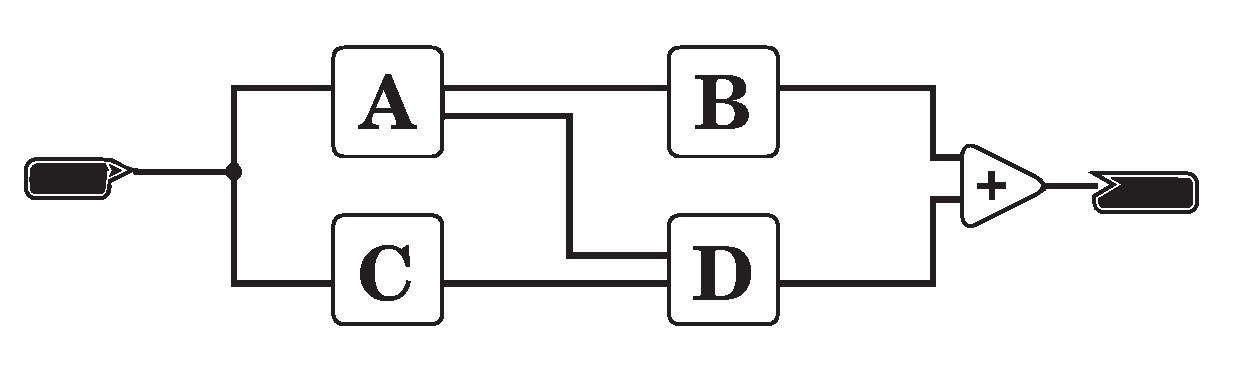
\includegraphics[width=150mm,keepaspectratio]{figures/vi1.pdf}
\caption{Dataflow program example} 
\label{fig:dataflowexample}
\end{figure}

\begin{lstlisting}[frame=single,float=!ht,caption={The same program using a procedural paradigm},captionpos=b,label={lst:proceduralexample},language=]
IN: i
(w1,w2) = A(i)
w3 = B(w1)
w4 = C(i)
w5 = D(w2,w4)
o = w3 + w5
OUT: o
\end{lstlisting}

I decided to convert the dataflow program to a procedural one, this means to define the execution order of nodes and turning the data flow wires into variables. This is possible, since executing a program in LabVIEW does the same - when running on the computer, the nodes execute in some order after each other. A node can execute, when all the input values are ready. This can also be observed in the development environment using the Highlight Execution tool, after executing a node the output values will slowly move to the next node. A G program cannot contain a wire cycle (except with feedback nodes), thus the nodes form a directed acyclic graph, which will have a topological ordering. When two or more topological ordering exist, it may be worth to choose the one that has forking statements later in the execution, to reduce execution time. Control structures will be quite easy to handle: case structures and loops are subdiagrams on a VI, and during conversion the contents of subdiagrams will become parts of If-Else statements and While loops. 

\section{Symbolic execution of a VI}

If performed correctly, the conversion will produce a simple algorithmic representation of the dataflow program. Symbolic execution can now be run.

From the symbolic execution point of view, VIs (Virtual Instruments) can be treated as the program, on which the symbolic execution is done. It has inputs, outputs, and most of the instructions are usually the native components of LabVIEW (so that their behaviour can be predicted). Controls are going to be the inputs, their data type can be chosen as one of the basic types, clusters (similar to struct), or objects. In the case of the symbolic execution tool, I am going to stick to the basic types. Indicators are the outputs of the program.

Instruction blocks use wires to pass data to each other. They are similar to variables in text-based languages, but they also define order of execution between blocks. Since each wire is going to represent a new variable in the program, the symbolic executor will have to deal with lots of unnamed variables.

Another issue is dealing with nodes that depend on external data source, or those that perform an operation that is not supported by the constraint solver.

\subsection{Program flow elements}
In the first prototype of the tool, I decided to implement the Case Structure only, 
\subsection{Arithmetical, logical, and other operations}

\section{Architecture}


\begin{figure}
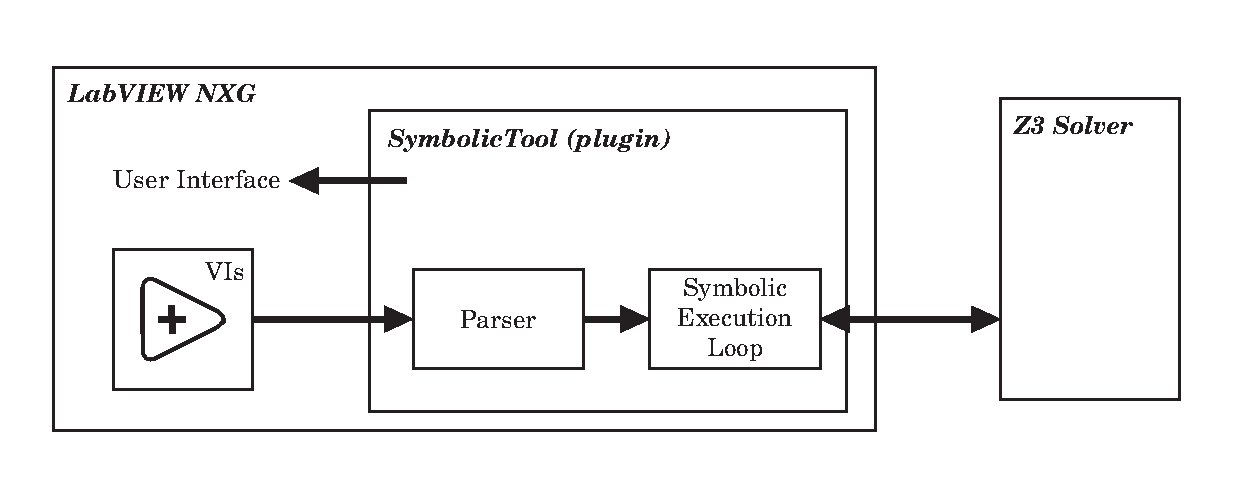
\includegraphics[width=150mm,keepaspectratio]{figures/architecture.pdf}
\caption{Architecture plan} 
\label{fig:architectureplan}
\end{figure}


The final architecture of the tool, based on the reasons above, will consist of the following:

\begin{itemize}
  \item Access the object model of the tested Virtual Instrument
  \item Generate a procedural representation of the dataflow program
  \item Execute the procedural program with the inputs of the VI as symbolic variables 
   \item Use a constraint solver to calculate the symbolic variables
in the leafs of the symbolic tree
     \item Display the calculated inputs (or use them to build a unit test)
  
  \end{itemize}

The first step depends entirely on the programming interface of NI software, so it will be a topic of the implementation section. Once the data model of the VI is accessible, it can be converted to a procedural program. To do this, an object model for the program has to be designed, which is tailored for the purpose of symbolic execution.

\subsection{Object model}

The starting point of the model will be the class \textit{Statement}, which is the same unit in the program as a node in the VI. These \textit{Statement}s will execute in a defined order, which is managed by a \textit{Sequence} object. \textit{Sequence} corresponds to the Block Diagram of the VI, or any subdiagram (in a case structure or a loop). Since a Node in the VI can do complex tasks, and have multiple outputs, a \textit{Statement} can be broken down to simpe instructions, \textit{Assignment}s, that evaluate an \textit{Expression}, and place the result in a \textit{Variable}.

\textit{Expression} is just an empty base class for the expression classes to derive from. This approach provides extensibility, any kind of expression can be treated the same way, and with the help of \textit{Operators}, complex expressions with two or more levels can be built.

\textit{IfStatement} and \textit{LoopStatement} will have \textit{Statement} as their ancestor to be able to join a \textit{Sequence}. The subdiagrams of a case structure or a loop will be a part of these \textit{Statement}s as \textit{Sequence}s.
\begin{figure}

\centering
\begin{tikzpicture}[node distance = 1cm, auto]
    % Place nodes
   
    
    \node [block] (seq) {Sequence};
    \node [block, below=of seq] (statement) {Statement};
    \node [block, below=of statement] (ifs) {IfStatement};
    \node [block, below right=of statement] (loop) {LoopStatement};
        
    \node [block, below left=of statement] (assignment) {Assignment};
    \node [block, below=of assignment] (expression) {Expression};
    \node [block, below left=of expression] (variable) {Variable};
    \node [block, below=of expression] (symvar) {SymbolicVar};
    \node [block, below right=of expression] (oper) {Operator};
    \node [block, right=of oper] (const) {Constant};
        
    \path [comp] (statement) -- (seq);
    \path [comp] (assignment) |- (statement);
     \path [generalization] (ifs) -- (statement);
     \path [generalization] (loop) |- (statement);
     \path [aggr] (expression) -- (assignment);
          \path [aggr] (variable) |- (assignment);
               
     \path [generalization] (variable) |- (expression);
     \path [generalization] (symvar) -- (expression);
     \path [generalization] (oper) |- (expression);
     \path [generalization] (const) |- (expression);
               
   % \node [block, below right=1cm and -2.6cm of arch] (des) {Detailed design};
    % \node [block_rounded, below right=1cm and -1cm of des] (dev) {Development};
  %  \node [block_rounded, above right=1cm and -1cm of dev] (utest) {Build and unit test};
 %   \node [block_rounded, above right=1cm and -2.6cm of utest] (itest) {System integration and test};
  %  \node [block_rounded, above right=1cm and -2.6cm of itest] (dep) {Deployment and verification};
    % Draw edges
 %   \path [line] (req) -- (arch);
  %  \path [line] (arch) --  (des);
  %  \path [line] (des) -- (dev);
  %  \path [generalization] (dev) -- (utest);
 %   \path [comp] (utest) -- (itest);
  %  \path [line] (itest) -- (dep);
  %  \path [double] (des) -- (utest);
   % \path [double] (arch) -- (itest);
   % \path [double] (req) -- (dep);
    
\end{tikzpicture}

\caption{Simplified diagram of the procedural program data model} 
\label{fig:datamodeldiagram}
\end{figure}



\section{Limitations}